\Transcb{yellow}{blue}{Why Neutrinos ?}
\twocolumn[\begin{center}{\blue Investigating the Universe with electromagnetic radiation}\end{center}]
\begin{center}
\includegraphics[keepaspectratio,width=5cm]{optical2}
\includegraphics[keepaspectratio,width=7cm]{radio2}\\[5mm]
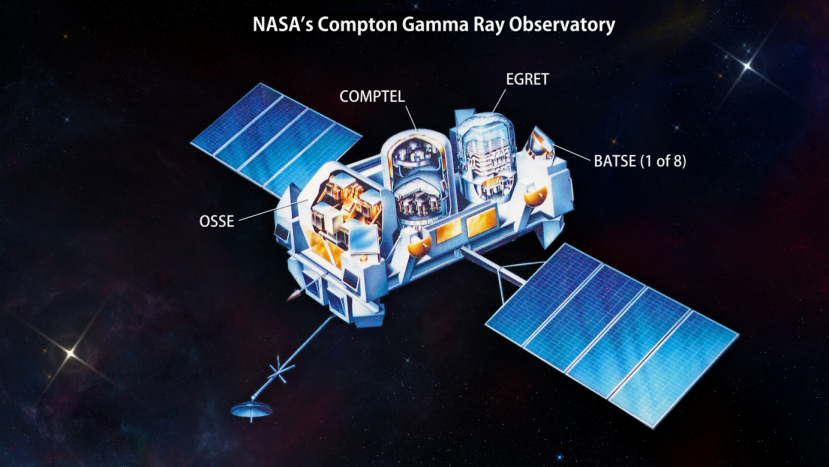
\includegraphics[keepaspectratio,width=13cm]{cgro2}\\
{\small [Credit NASA]}
\end{center}

\newpage

\begin{center}
\includegraphics[keepaspectratio,width=13cm]{milky-way}
\end{center}
%
\begin{itemize}
\item[] \colorbox{yellow}{Observations at different wavelengths}
\item Various new discoveries (pulsars)
\item Better insight in (astro)physical\\
      processes
\item Rather complete view on the large\\
      picture of the Universe
\end{itemize}

\Tr
\twocolumn
\begin{center}
{\blue Observed jet signature} (M87)\\[2mm]
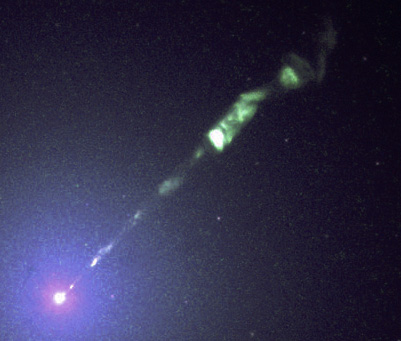
\includegraphics[keepaspectratio,height=12.5cm]{M87jet}\\
{\small [Credit NASA]}\\[2mm]
\colorbox{yellow}{Acceleration in shock waves}
\end{center}

\newpage

\begin{center}
{\blue Processes in the jet}\\[5mm]
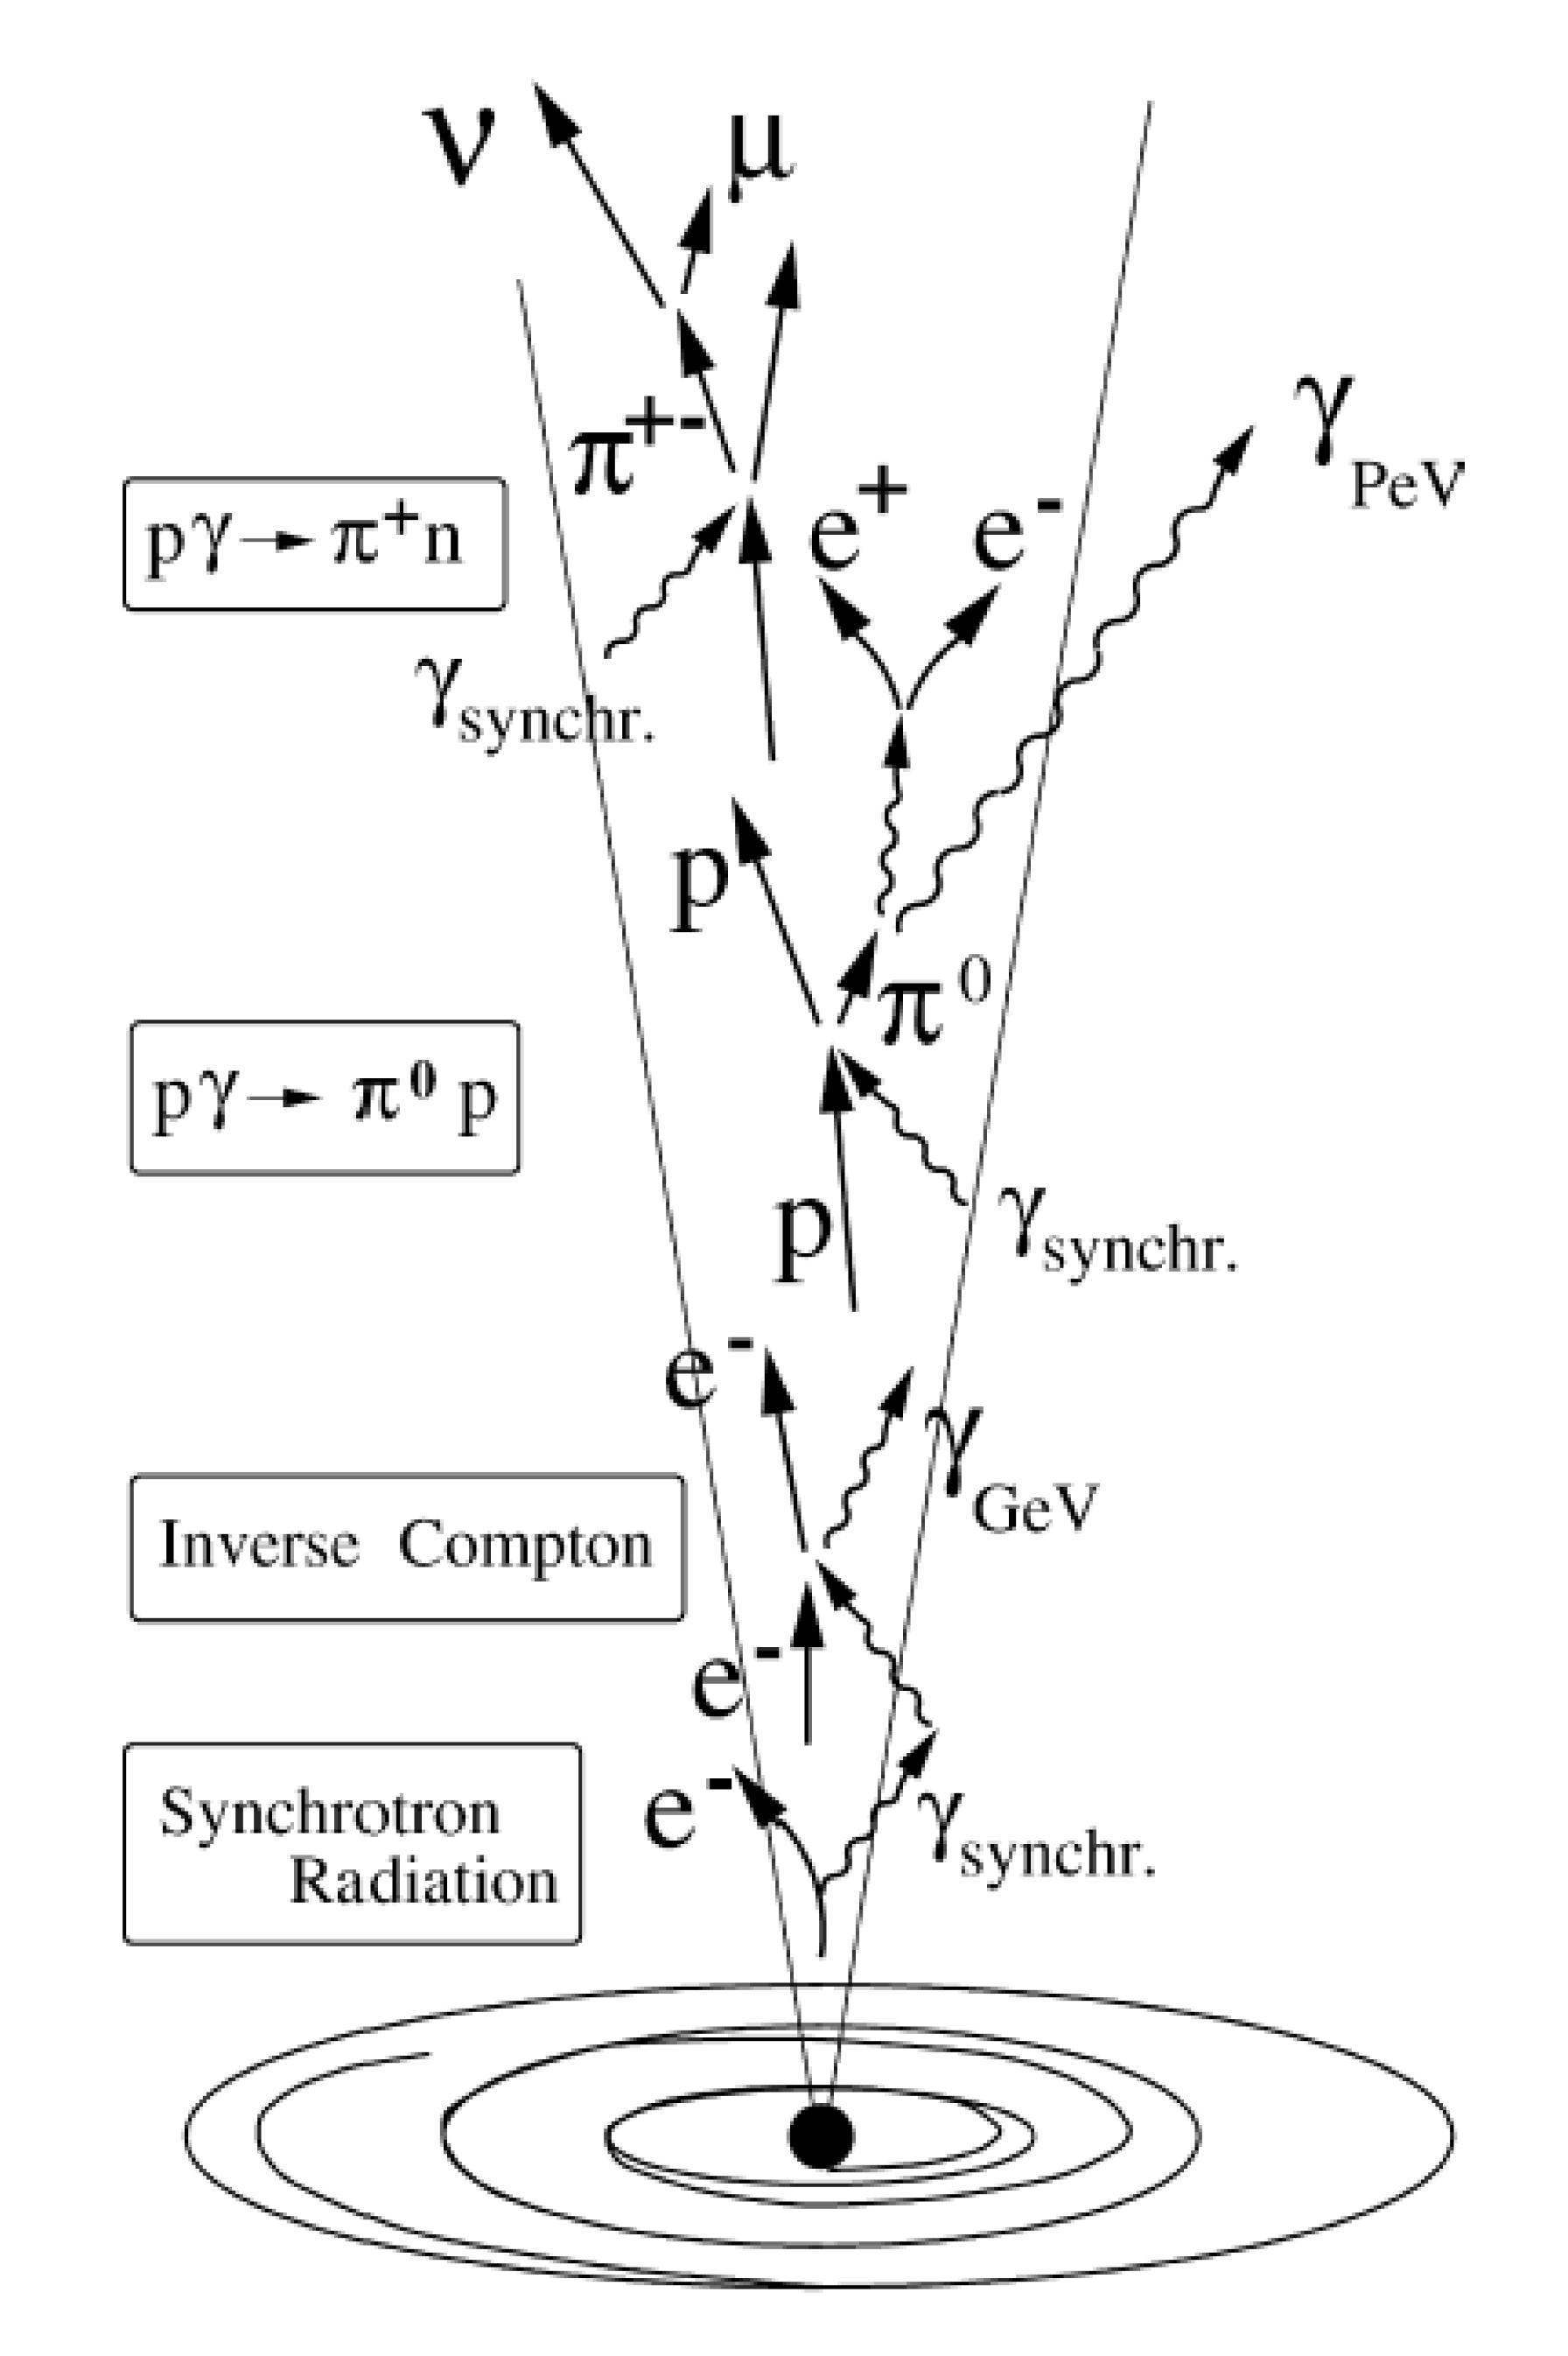
\includegraphics[keepaspectratio,height=12.3cm]{jet}\\
{\small [Credit C. Spiering]}\\[2mm]
\colorbox{yellow}{High-energy $\gamma$, nuclei and $\nu$}
\end{center}

\Tr
\twocolumn
\begin{center}
\includegraphics[keepaspectratio,height=15.7cm]{app-vertical}
\end{center}

\newpage

\begin{center}
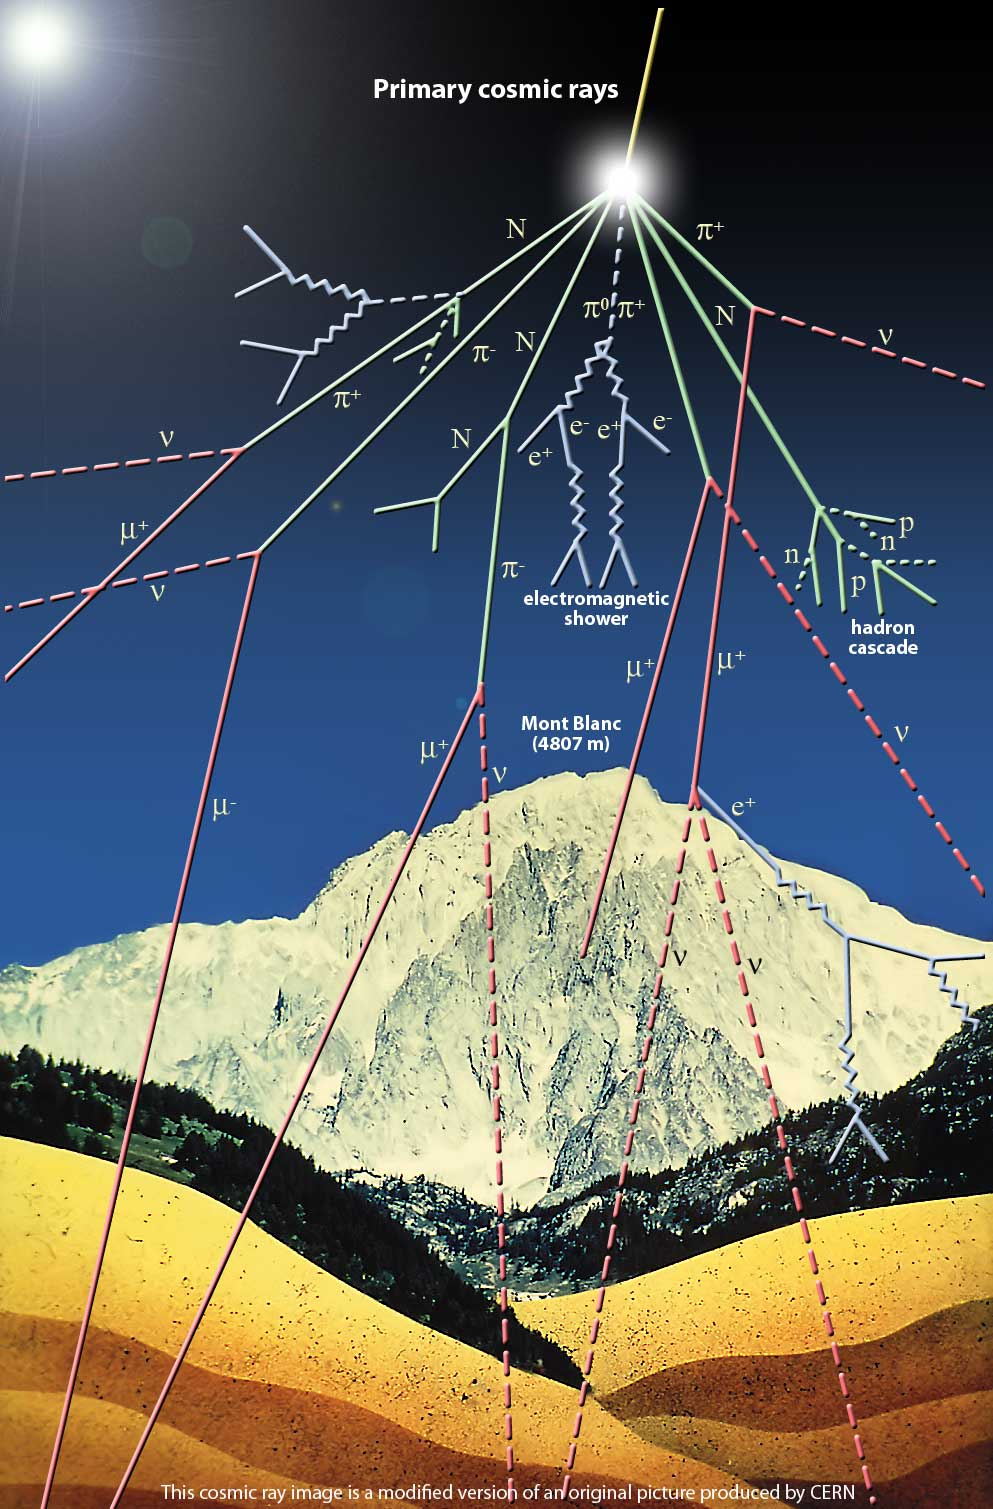
\includegraphics[keepaspectratio,height=15.7cm]{cosray}
\end{center}

\Tr
\twocolumn
\vspace*{2mm}
\begin{center}
{\blue The $E^{2.6}$ scaled Cosmic Ray flux}\\[3mm]
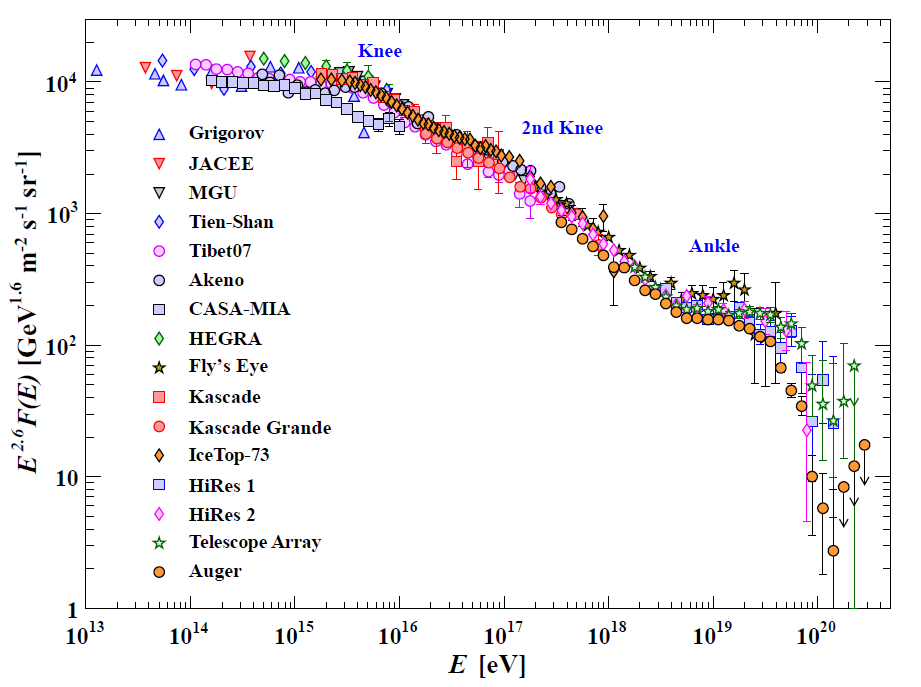
\includegraphics[keepaspectratio,width=14cm]{cr-all-scaled26}\\
{\small [Credit PDG 2014]}
\end{center}

\newpage

\vspace*{3cm}
\begin{itemize}
\item Spectral features (knee, ankle)
\item[] $E$ limits of cosmic accelerators~?
\item[] Onset of extra-galactic component~?
\item[] Do we observe the GZK cut-off ?
\item Cosmic Rays already detected in 1912
\item[] {\blue Sources still not identified}
\end{itemize}

\Tr
\onecolumn
\begin{center}
{\blue Beware of the observable Universe:
 $\gamma+\gamma_{EBL}\rightarrow e^{+}e^{-} \qquad N+\gamma_{CMB} \rightarrow \Delta$}\\
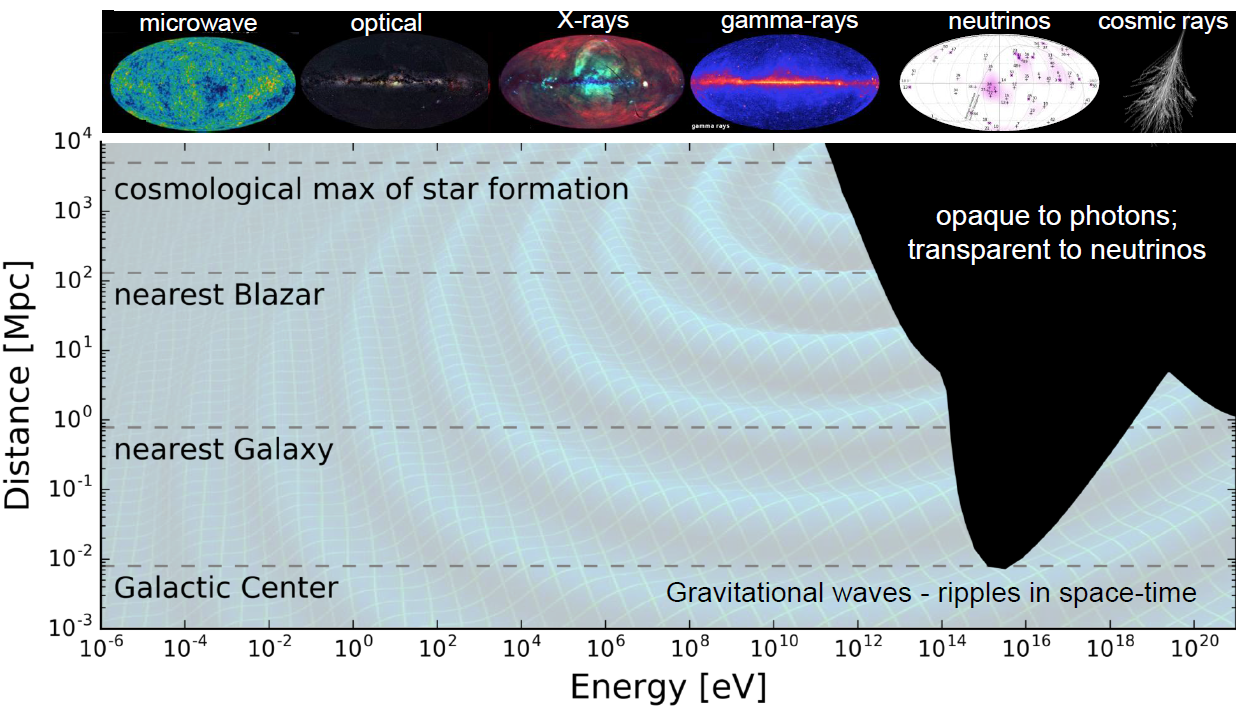
\includegraphics[keepaspectratio,height=14cm]{marek}\\
{\large [Credit Marek Kowalski]}
\end{center}

\Tr
\twocolumn
\begin{center}
\colorbox{yellow}{Neutrino production mechanism}\\
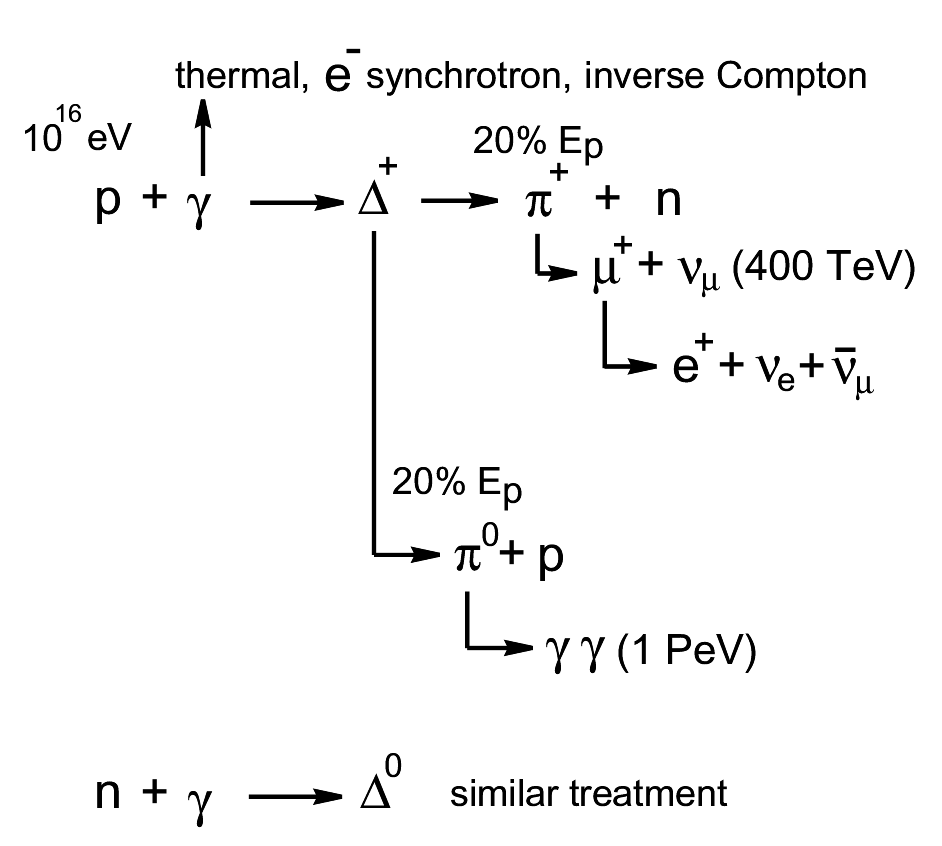
\includegraphics[keepaspectratio,width=13cm]{grb-engine2}
\end{center}
%
\begin{itemize}
\item $\Delta$ prod. threshold~: $E_{\gamma} \ge 10$ eV\\
      (UV photons)
\end{itemize}

\newpage
%
\begin{itemize}
\item {\red Waxmann-Bahcall} {\large [PRL 78 (1997) 2292]}
\item[] High-E $p$ diffuse out of the shocks
\item[] Observed CR $\rightarrow$ lower limit on $p$ flux 
\item[] {\blue Fraction of $p$ used for $\nu$ production ?}
\item {\red M. Ahlers et al.} {\large [APP 35 (2011) 87]}
\item[] Protons trapped, neutrons escape
\item[] CR observations provide the $n$ flux
\item[] {\blue Direct relation CR $\leftrightarrow \nu$ flux}
\item {\red Generic $\nu$ spectrum} {\large [JCAP 0903 (2009) 020]}
\item[] 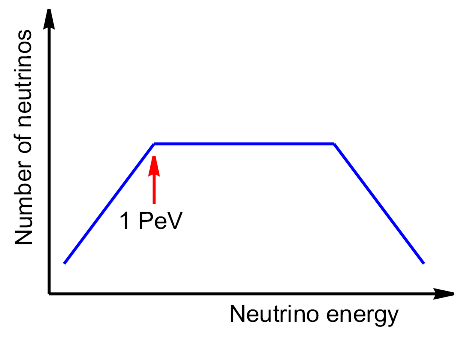
\includegraphics[keepaspectratio,height=6cm]{wb-spectrum}
\end{itemize}

\Tr
\twocolumn
\begin{center}
\includegraphics[keepaspectratio,height=15.7cm]{app-vertical}
\end{center}

\newpage

\begin{center}
{\blue Neutrino detection principle}\\
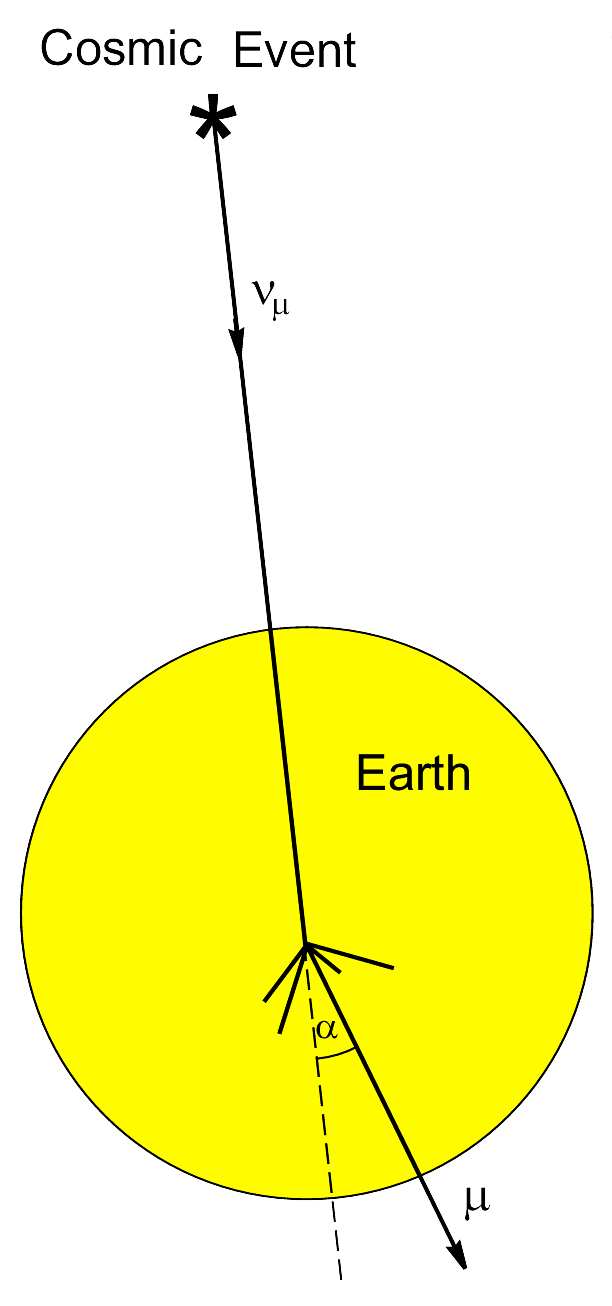
\includegraphics[keepaspectratio,height=14.7cm]{earth-shield}
\end{center}
